\chapter{Evaluation}\label{chapter:eval}
In previous chapters, we introduced the design and implementation of 2 prototype
video recommendation applications, MiRec and DiRec, that are developed for the
purpose of testing the effect of distributing the UI of a single user recommender system on the users'
experience; whether this distribution will enrich and facilitate users'
experiences of such systems or would be considered redundant or confusing. To
put this to test, we designed a closed user study, in which participants were
asked to interact with and use both prototype applications, and then give their
feedback evaluation through a user experience survey directly after they are done with
using the apps. In this sections, we explain the different phases of the user
study. We also explain our evaluation method, as well as present the results of
the analysed user experience survey collected from the study participants.

\section{User Study Phases}
The overall goal of the study is to elicit the users’ direct
feedback and impressions of their experience of using the prototype apps.
Each of the phases described below will have its own sub-goal that works
towards this main goal. The study is divided into 3 phases. It starts in a
usability demo in which we demonstrate to participants how to use the apps,
which we thought is necessary to avoid any confusion which might affect the
users rating of the app and tamper with their evaluations. Phase 2 is the actual
user test in which participants interact and use the apps. And the final phase
is the post-experiment user experience survey which is done shortly after phase
2. In the course of 2 weeks, participants were invited to use our apps and give
their feedback. We started our evaluation of the collected user feedback shortly
after we had sufficient number of participants that lead to a stable evaluation.
The following are details of each phase of the study as well as a presentation
of the results and how we interpret them.
\subsection{Phase 1: Usability Demo}
The goal of this phase is to explain clearly to participants the functionalities
of both prototypes. According to the participant’s background, information about
recommender systems, their goal and how they work, were provided. We started by
explaining to participants what tasks are expected to be completed by the them.
We explained that both apps function similarly except that with DiRec, some
functionalities could be done on the phone and others could be transferred to
the screen. We then proceeded with demonstrating to the participant what they
could do with each app. In MiRec, we explained how to play and rated videos, how
to view the video details, and how to navigated through the list of
recommendations in the Home screen as well as through the categories. In DiRec,
we also demoed what could be done on the phone and what could be done on the
screen. The gestures of swipe-left to view details on screen, swipe-right to
filter, and pan on video photo to play on screen were also demoed clearly so
participants would know how to perform the tasks. We explained that the goal of
the study is not to test the functionalities but to get their impression about
the apps. After all fucntionalities were demoed, participants were handed in a
sheet that has the tasks they are expected to complete written down in the form of steps (see appendix). Also, they were
handed in the user-experience questionnaire sheets. Participants were asked to
take their time and ask any questions if needed and to fill-in the questionnaire
directly after they are done.
\begin{figure}[t]
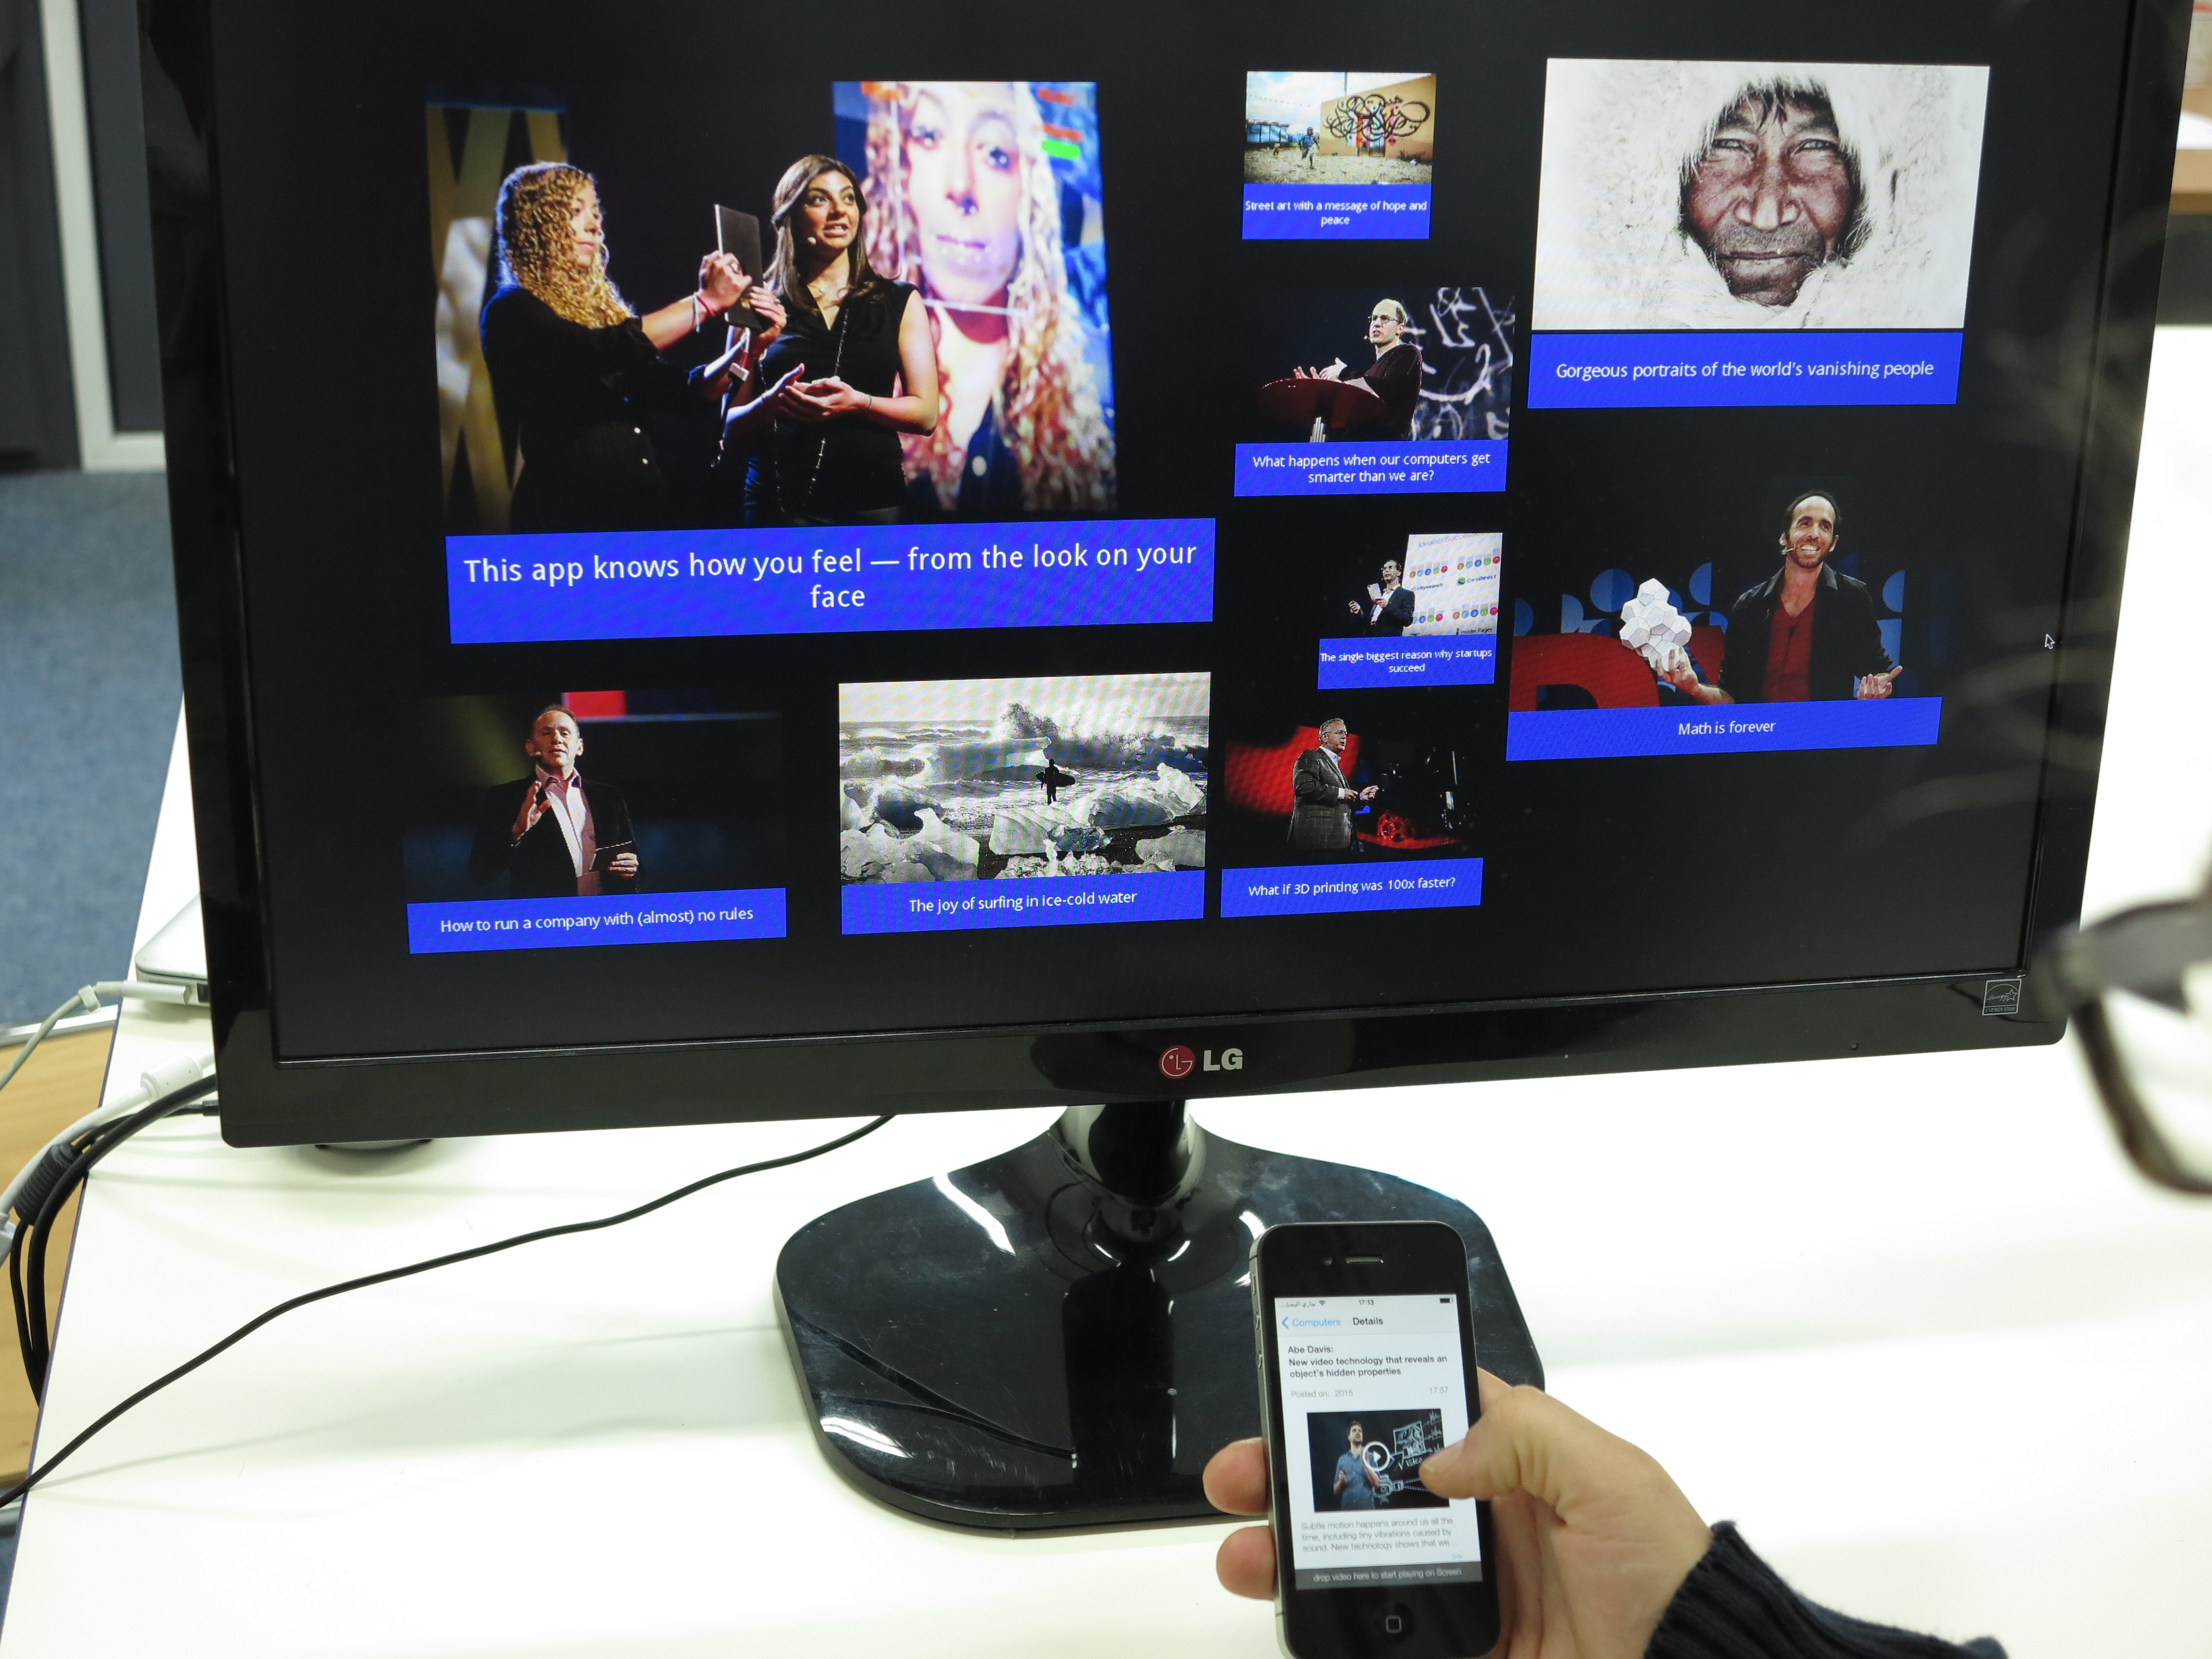
\includegraphics[width=0.75\textwidth, center, center]{figures/IMG_6806}
\caption{Participant's interaction with DiRec during the study.}
\label{fig:figure51}
\end{figure}
\subsection{Phase 2: Prototypes' Functionalities Test}
The user test was done after the participant was made familiar with the apps and
with the tasks of the study. Figure \ref{fig:figure51} shows part of one of the
participant's interaction with DiRec during phase 2 of the user study. Each
participant was given an iPhone mobile device with MiRec and DiRec installed, and was asked to sit across of an LD screen, which works as a display to DiRec's LD component.
Participants were asked to start with the app version of their choice to avoid
bias. After they are done with a given version, they start the tasks of the
second version. The tasks were put in place so as to have a standard set of
steps that all participants do. These steps (appendix) mainly consist of:
navigating the list of recommendations through the Home screen, viewing video details, playing
a video, rating a video, selecting a category of choice from the side menu, and
for DiRec, filtering was added to this list. By the end of each set of steps in
each app, we note that optionally users could then proceed interacting with the
apps for whichever scenarios they have in mind. Participants were informed that
this session would on average take between 15 to 20 minutes but they were also
asked to take their time or to stop the experiment at any time if they feel they
are already done and have a feel of the apps already formed. Participants were
observed during this test session, as part of the evaluation is to see how users react to the distribution aspect of the app.
Our observations of participants' interactions constitute part of our evaluation
of the results as shown later in the result section.
\begin{figure}
    \centering
    \begin{subfigure}[b]{0.3\textwidth}
        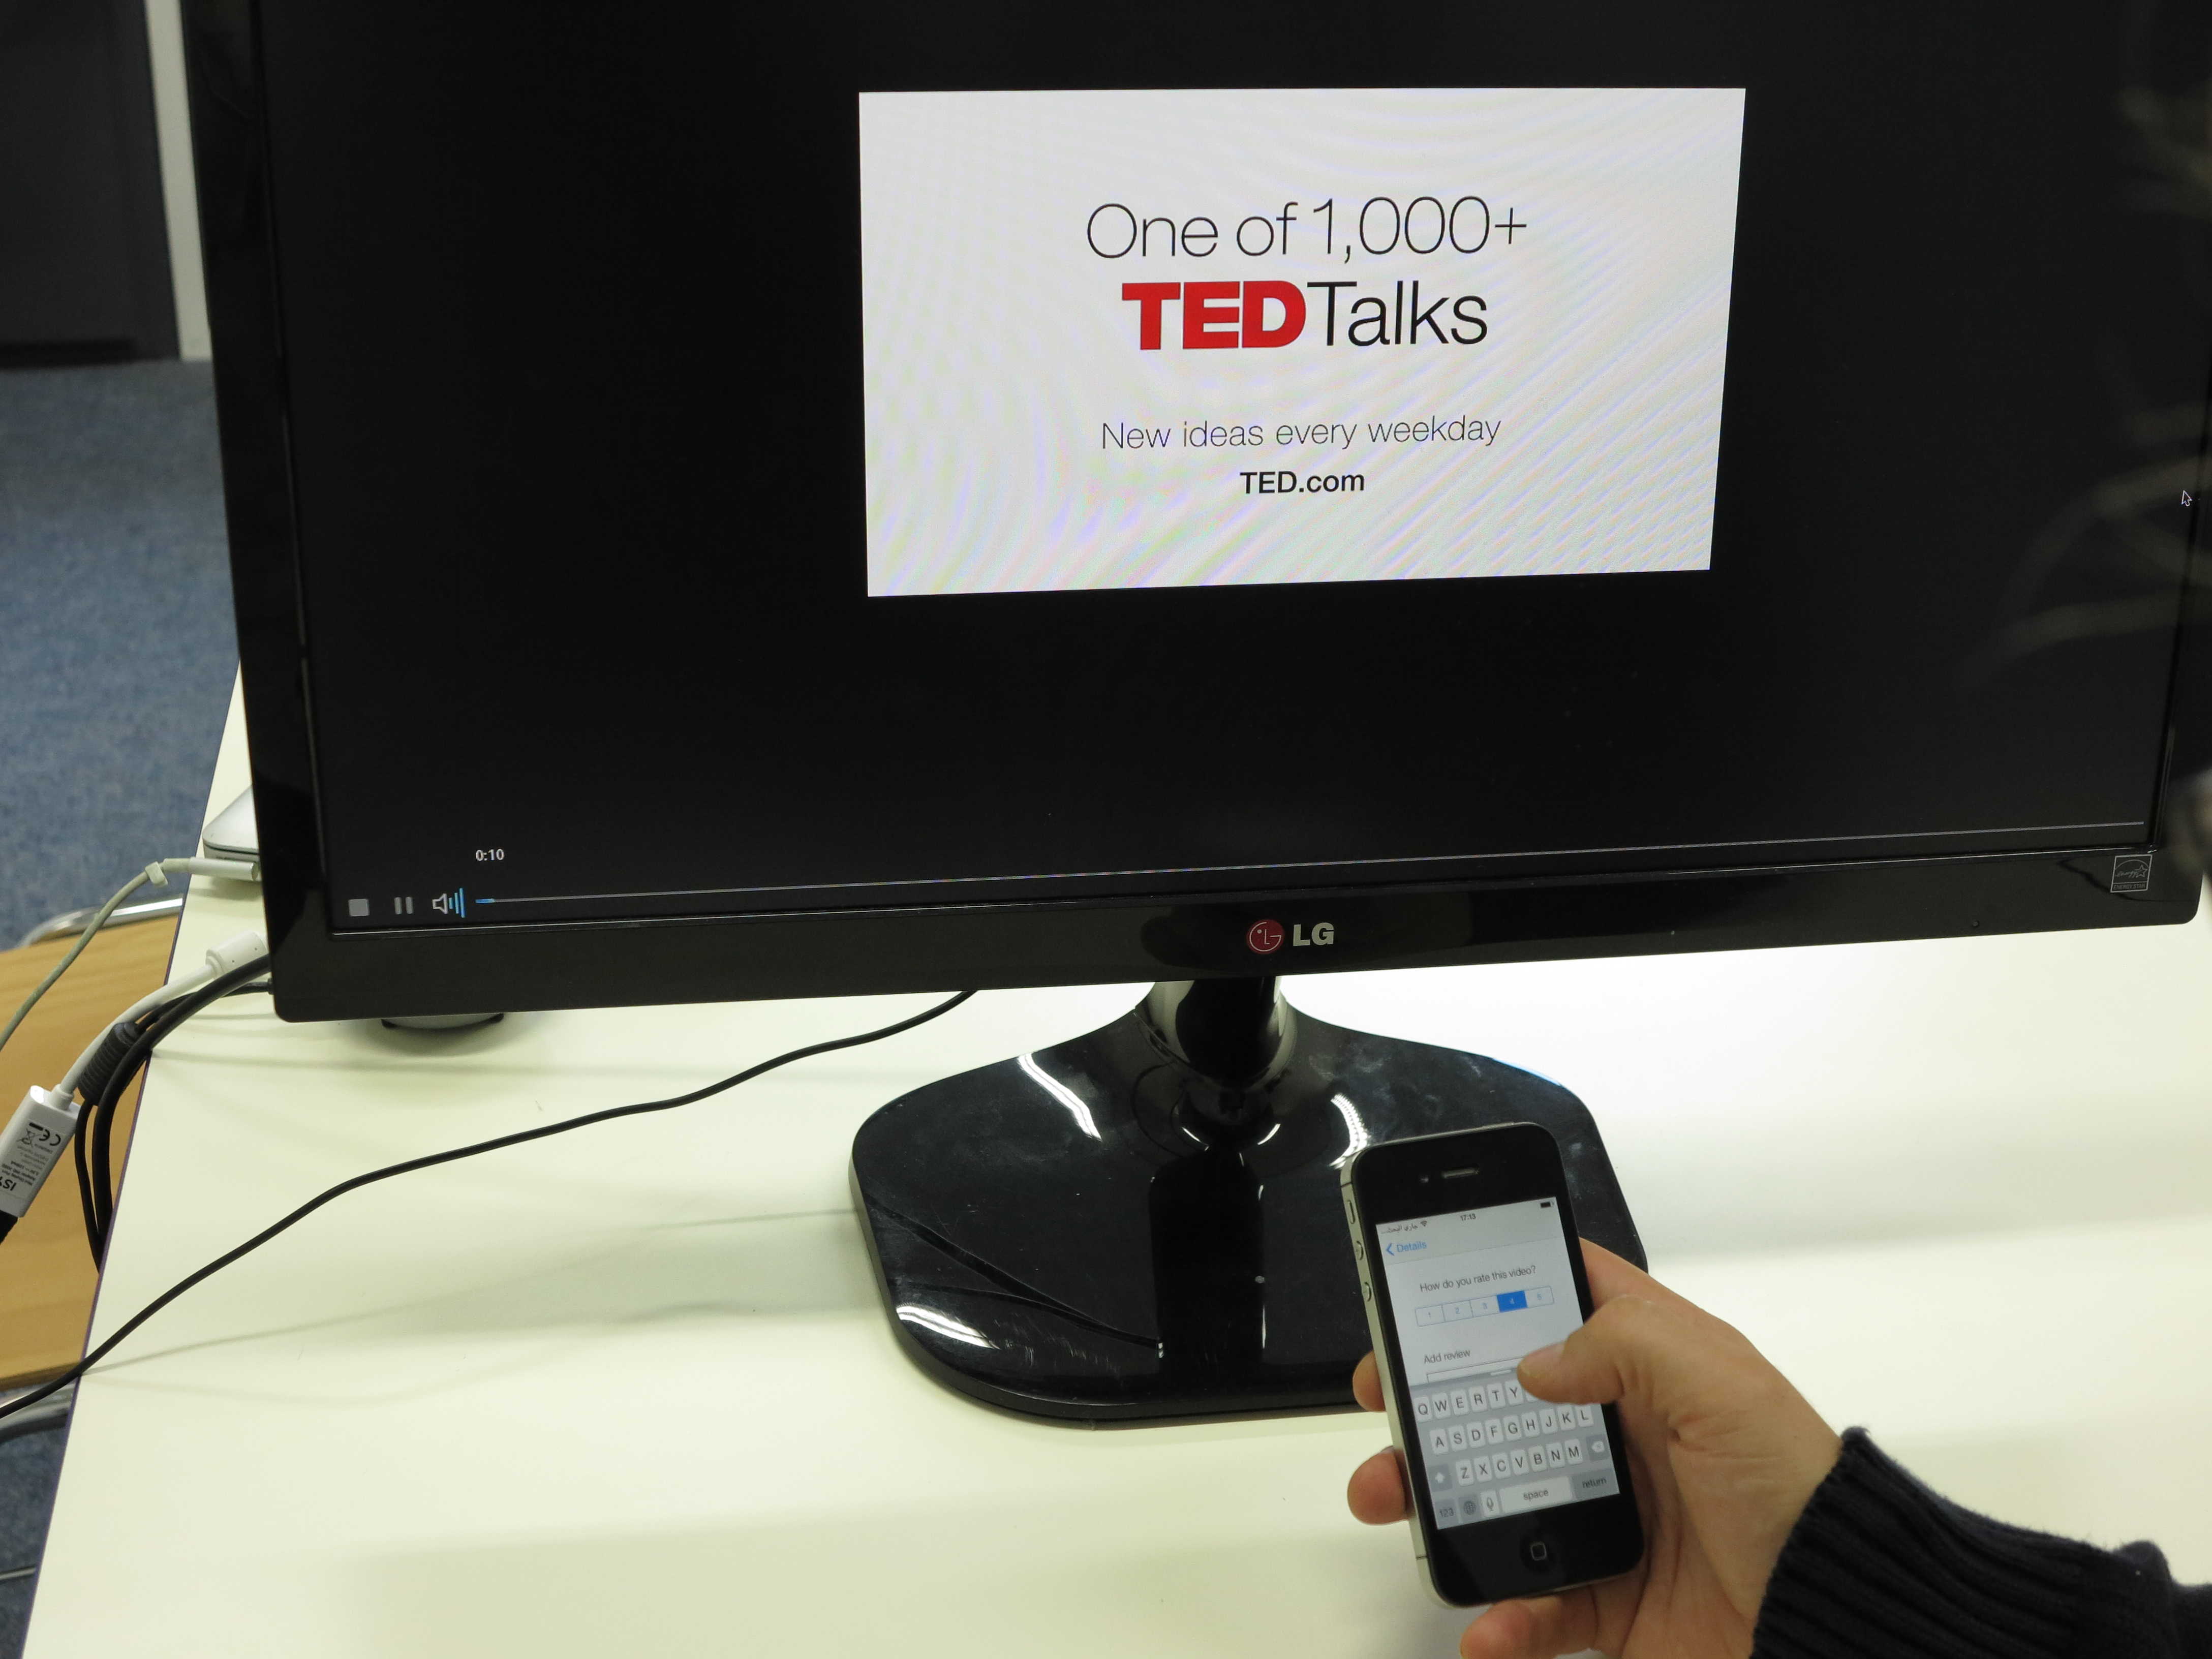
\includegraphics[width=\textwidth]{figures/IMG_6807}
        \caption{Rating and playing a video.}
        \label{fig:figure52a}
    \end{subfigure}
   
    \begin{subfigure}[b]{0.3\textwidth}
        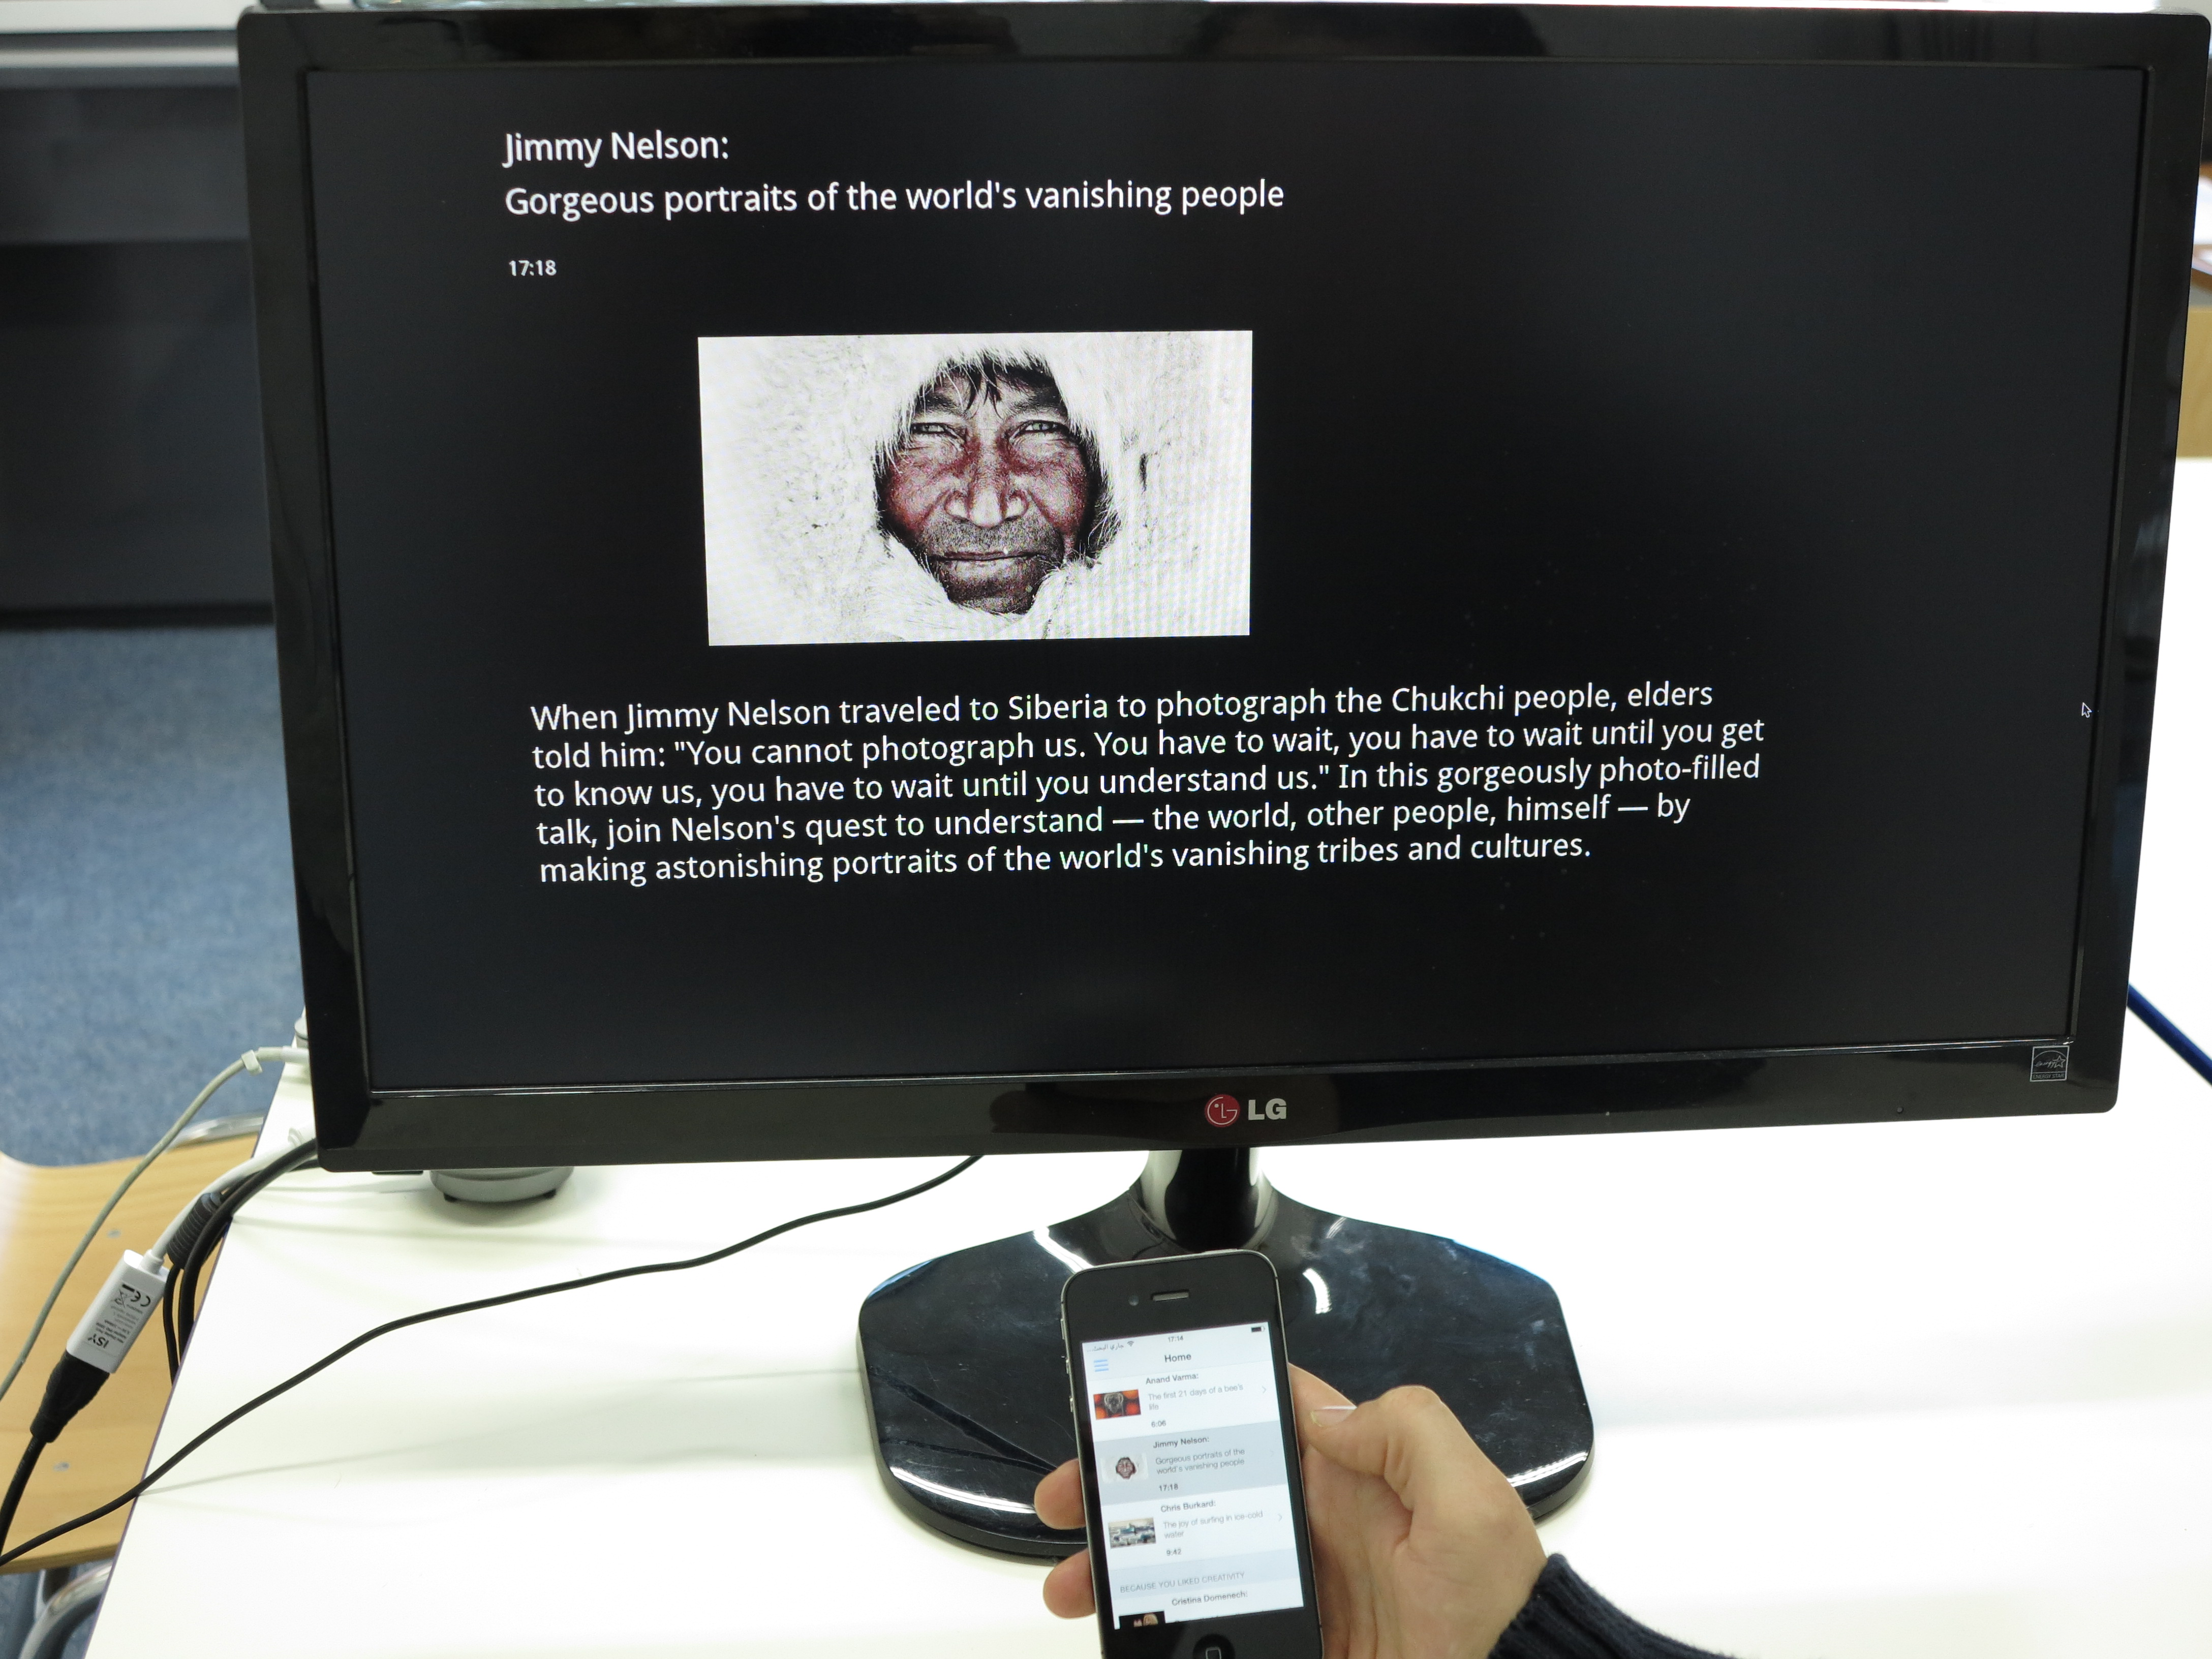
\includegraphics[width=\textwidth]{figures/IMG_6809}
        \caption{Viewing video details on DiRec}
        \label{fig:figure52b}
    \end{subfigure}
    
    \begin{subfigure}[b]{0.3\textwidth}
        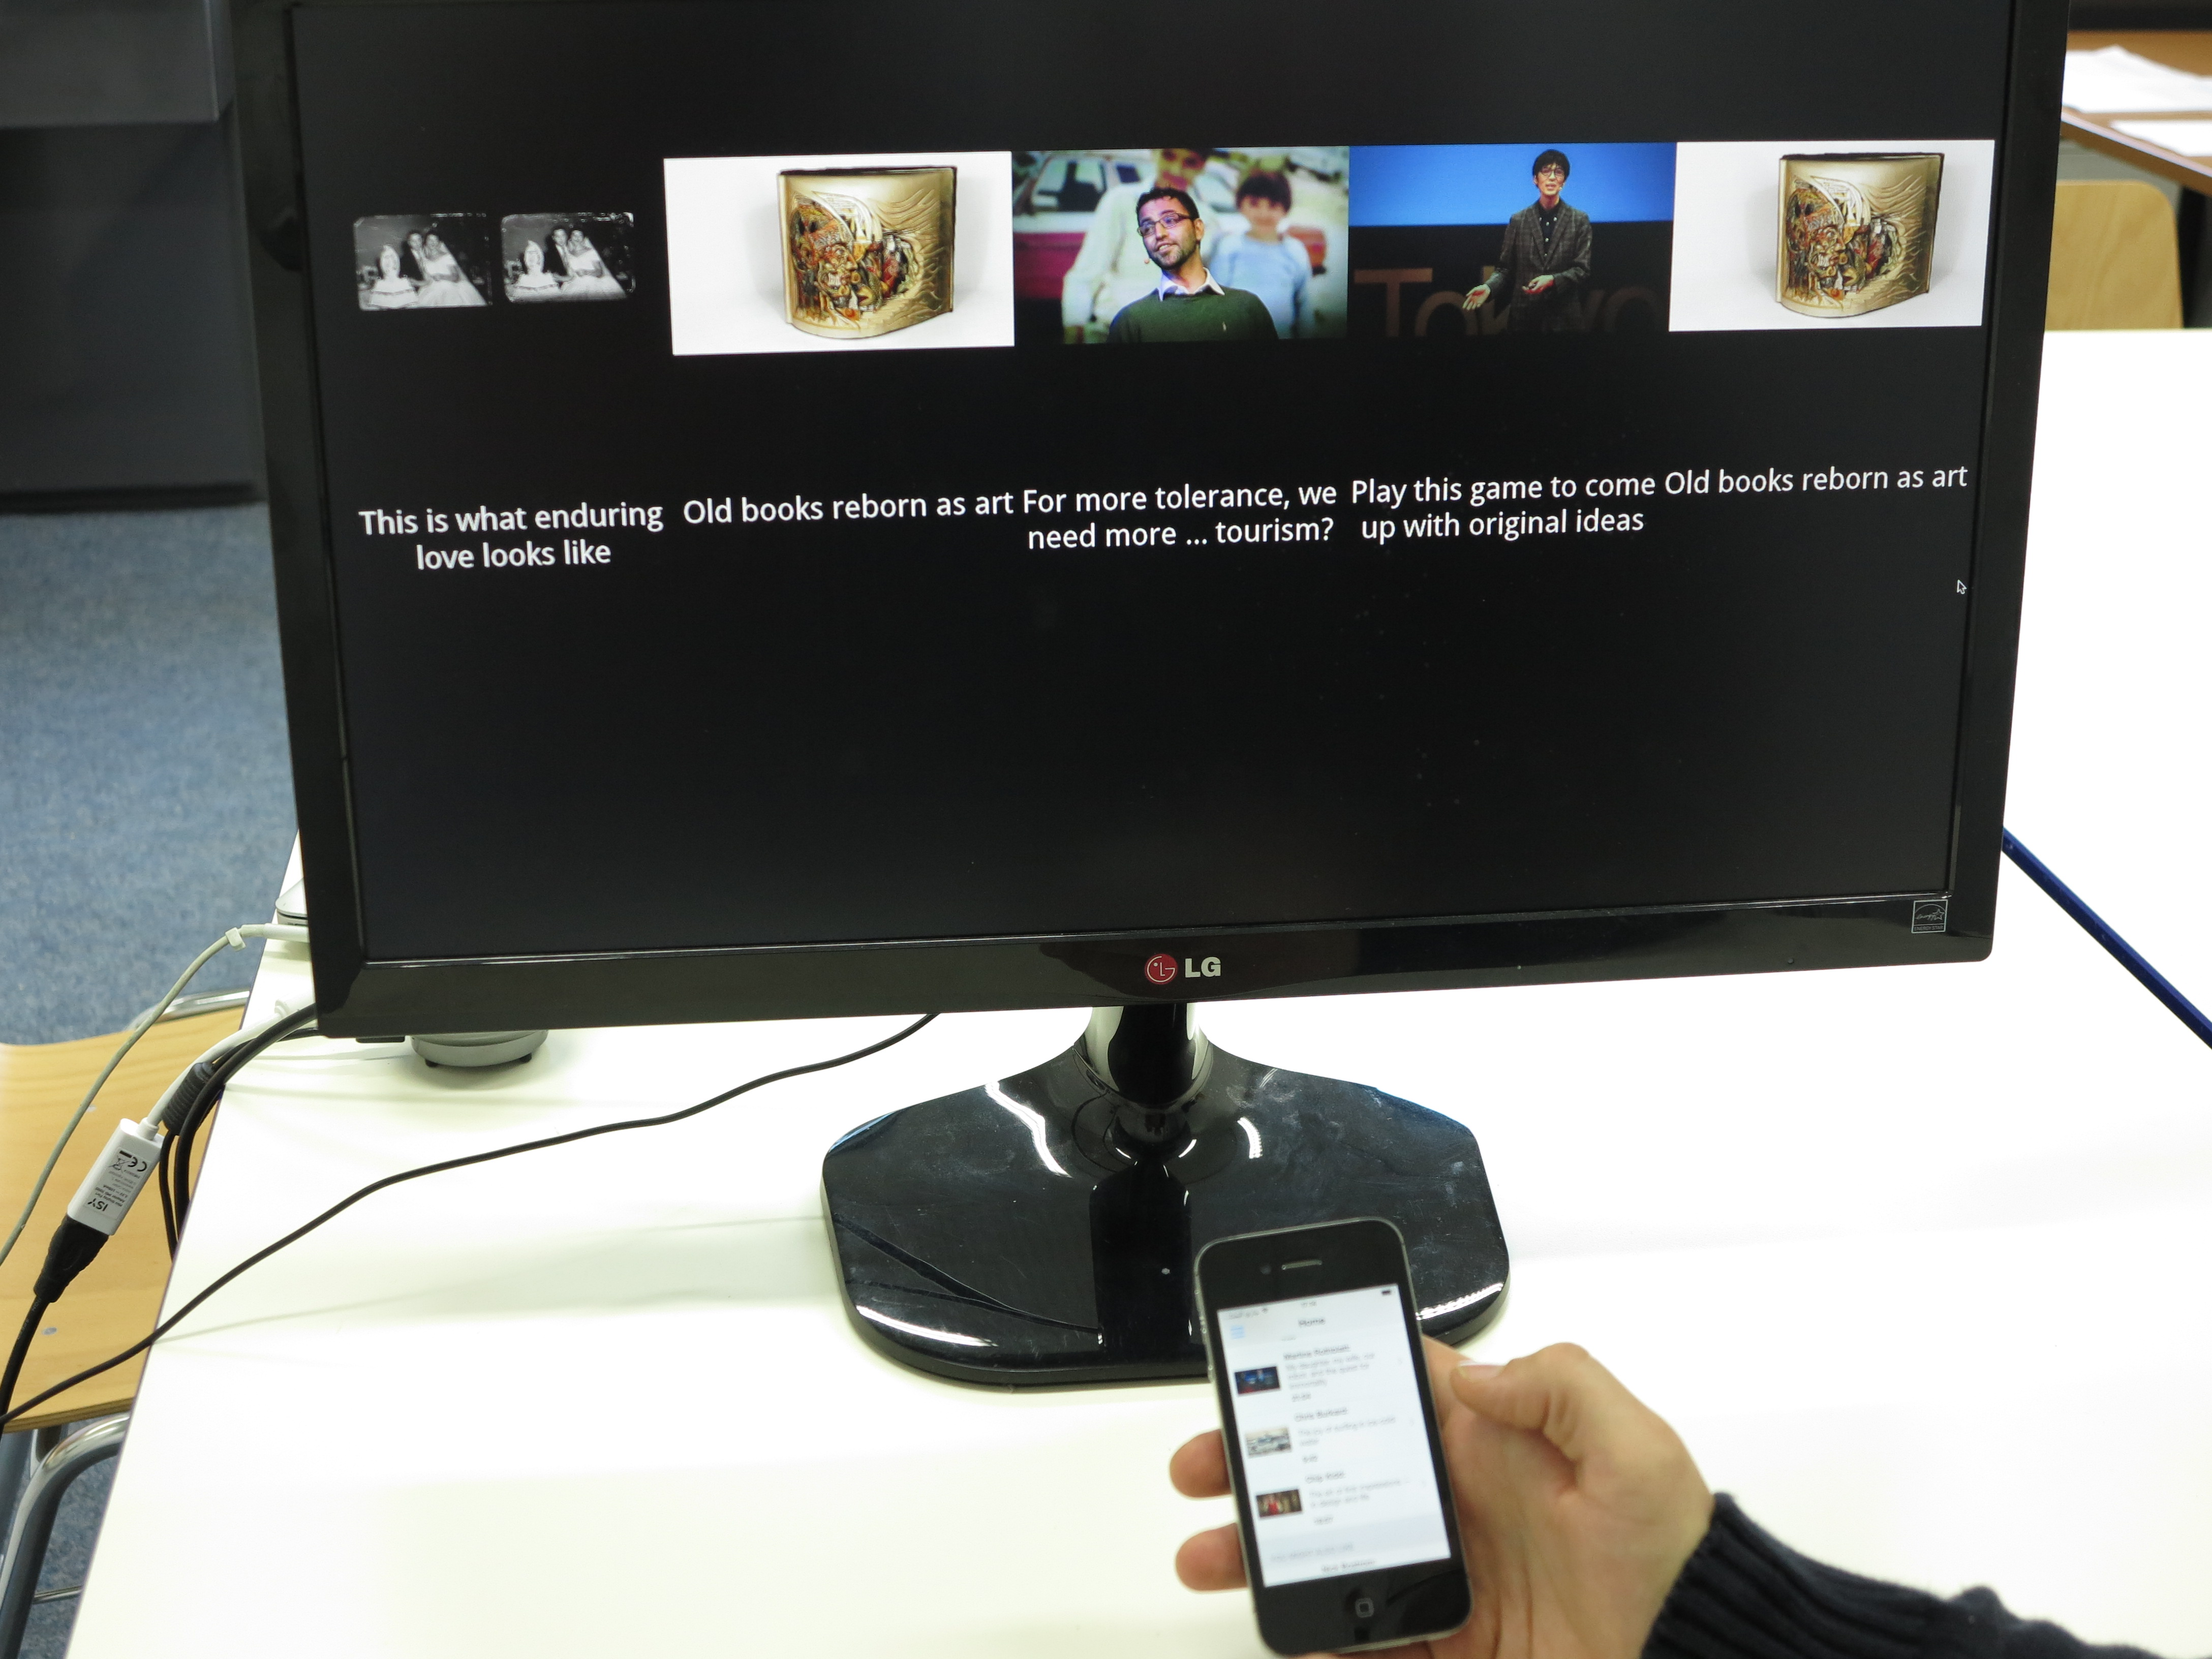
\includegraphics[width=\textwidth]{figures/IMG_6810}
        \caption{Filtering videos}
        \label{fig:figure52c}
    \end{subfigure}
   \caption{Interacting with DiRec.}\label{fig:figure52}
\end{figure}
 
\subsection{Phase 3: Post-Experiment Survey}
For eliciting participants' feedback, we use the User Experience Questionnaire
(UEQ) suggested by Laugwitz et al.
\cite{laugwitz2008construction}. This questionnaire is designed to elicit users
direct impression through rating of a set of 26 different attributes of the
apps on a scale from 1 to 7. For the study, each participant was given 2
sheets of the UEQ test and was asked to give their ratings for each app
separately, directly after she/he is done with using the apps. She/He were also
asked to not take more than 3 to 5 minutes in each evaluation, and not to analyse her
answers, as the goal is to get her overall direct impression. Appendix
show all of the 26 aspects that users were to rate. Participants were also asked
to write down their overall feedback and comment in textual form in case they
have any. Some participants preferred to give their feedback directly to us
verbally after the study was complete. We took the change to also interview some
of the participants and ask them about what she/he liked or disliked
specifically about the apps which was valuable to our analysis. Details of our
post-experiment interviews are given in the results section.

\section{Participants Demographics}
23 participants joined our study, non of which are involved directly or
indirectly in this research.
Of the 23 participants, 18 are males and 5 are females. The age range of
participants is between 23 to 31. The majority of the participants are masters
of informatics students at TU Munich, some are researchers or developers in the
same field. We assumed that all participants have no prior knowledge in
recommender systems and explained the procedure similarly to everyone regardless
of their level of expertise.

\section{Study Results}

%\begin{figure*}[t]
%\centering
%\includegraphics[width=1.0\textwidth]{figures/comparison.pdf}
%\caption{Comparison of Scale Means in MiRec and DiRec.}
%\end{figure*}


%\begin{table}[]
%\centering
%\begin{tabular}{|l|l|l|l|l|l|l|l|l|l|l|l|l|l|}
%\hline
%\multicolumn{1}{|c|}{\multirow{2}{*}{\textbf{Scale}}} &
% \multicolumn{5}{c|}{\textbf{MiRec Dataset}}                                                &                        &  & \multicolumn{6}{c|}{\textbf{DiRec Dataset}}                                                                         \\ \cline{2-14} \multicolumn{1}{|c|}{}                                & \textbf{Mean} & \textbf{STD} & \textbf{N} & \textbf{Confidence} & \multicolumn{2}{l|}{\textbf{Confidence Interval}} &  & \textbf{Mean} & \textbf{STD} & \textbf{N} & \textbf{Confidence} & \multicolumn{2}{l|}{\textbf{Confidence Interval}} \\ \hline
%\textbf{Attractiveness}                               & 1.48          & 0.89   
% & 21         & 0.38                & 1.09                     & 1.86                   &  & 1.94          & 0.88         & 19         & 0.39                & 1.55                    & 2.33                    \\ \hline \textbf{Perspicuity}                                  & 2.11          & 0.93         & 21         & 0.40                & 1.71                     & 2.51                   &  & 1.00          & 1.34         & 19         & 0.60                & 0.40                    & 1.60                    \\ \hline
%\textbf{Efficiency}                                   & 1.74          & 0.78   
% & 21         & 0.34                & 1.40                     & 2.07                   &  & 1.58          & 1.07         & 19         & 0.48                & 1.10                    & 2.06                    \\ \hline \textbf{Dependability}                                & 1.11          & 0.76         & 21         & 0.32                & 0.78                     & 1.43                   &  & 0.97          & 1.03         & 19         & 0.46                & 0.51                    & 1.44                    \\ \hline
%\textbf{Stimulation}                                  & 0.83          & 0.83   
% & 21         & 0.36                & 0.48                     & 1.19                   &  & 1.67          & 1.10         & 19         & 0.49                & 1.18                    & 2.16                    \\ \hline \textbf{Novelty}                                      & -0.27         & 1.18         & 21         & 0.50                & -0.78                    & 0.23                   &  & 1.80          & 0.74         & 19         & 0.33                & 1.47                    & 2.14                    \\ \hline
%\end{tabular}
%\caption{Comparison of Scale Means Shows the scale means and the corresponding
% 5 percent confidence intervals.}
%\label{resTable1}
%\end{table}


UEQ handook \cite{UEQHandbook}
